\chapter{Centre Shipment}
\label{chap:centre-shipment}

Shipments allow for specimens or containers to be transferred from one centre
to another. E.g. collecting centres send to processing centres, storage centres
send to request centres, etc. Figure \ref{fig:centre-shipment} shows that
shipments are managed by the \entitylink{Centre} aggregate root.

\begin{figure}[H]
  \centering
  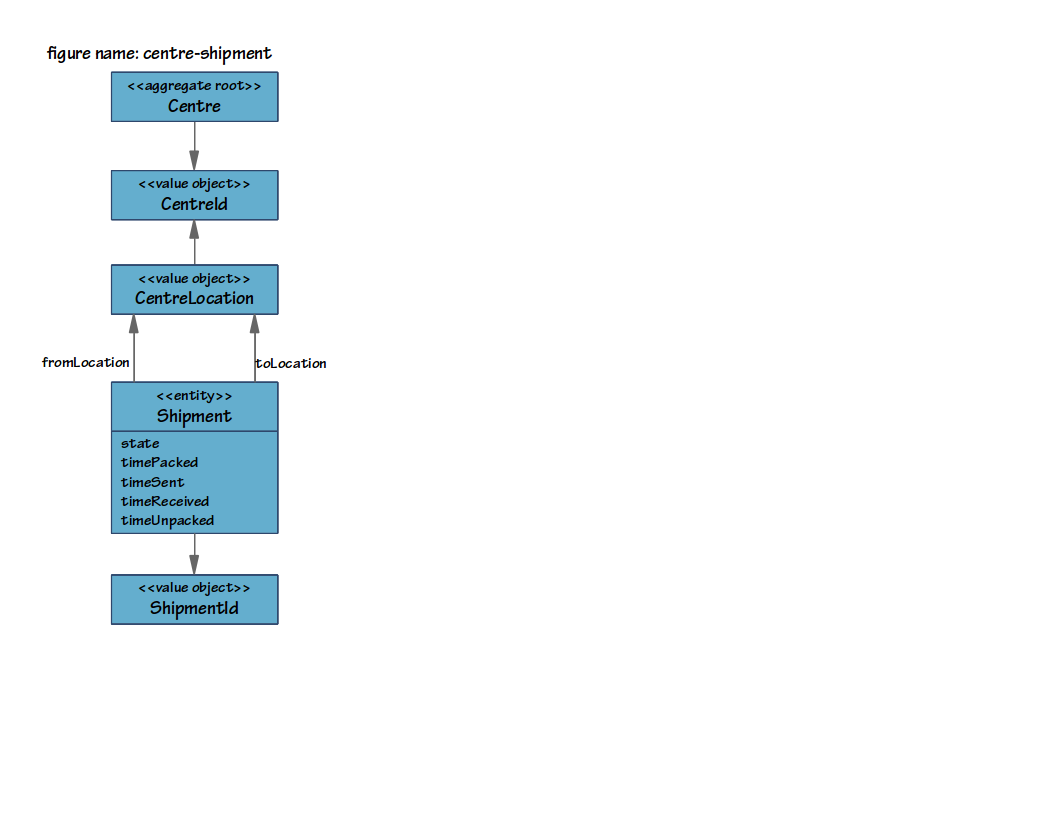
\includegraphics[trim={10mm 42mm 190mm 18mm}, clip,
    width=0.3\textwidth]{images/centre-shipment}
  \caption{Shipment Entity}
  \label{fig:centre-shipment}
\end{figure}

Since a centre could have multiple locations, \entitytarget{Shipment}s have a
\compfont{fromLocation} and a \compfont{toLocation} which identify the two
\entitylink{Centre}s involved. Both these centres must be enabled for the
shipment to be allowed.

A shipment has one of the following states:
\begin{statetable}
  CREATED & The shipment is in the process of being created.\\

  PACKED & The shipment is put together in a box, but not sent out.\\

  SENT & The shipment has been sent (possibly by a courier) to its destination.\\

  RECEIVED & The shipment has arrived at its expected destination, but has not
  been unpacked.\\

  UNPACKED & The shipment has arrived and its contents were confirmed.\\

  LOST & The shipment never arrived and may never arrive.\\
\end{statetable}

The shipment also records when the shipment was packed, sent, received and
unpacked. These are recorded as date and time stamps. Figure \ref{fig:shipment}
shows the remainder of the model for shipments.

\begin{figure}[H]
  \centering
  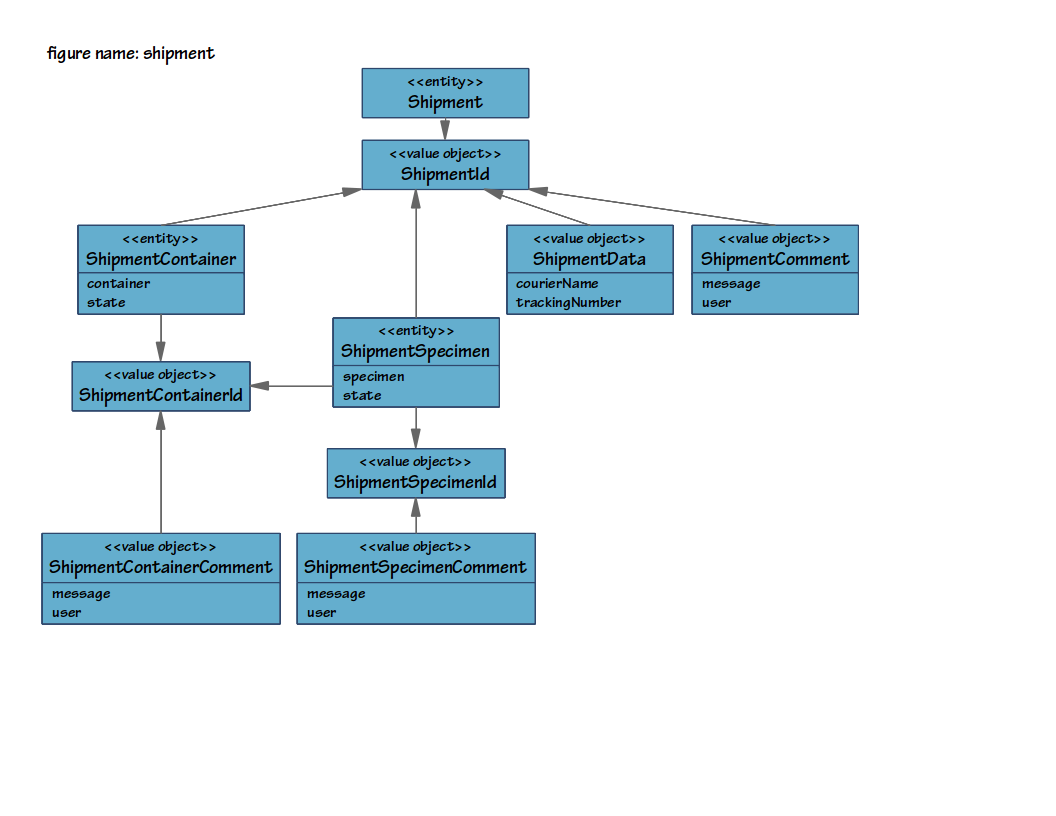
\includegraphics[trim={10mm 46mm 50mm 18mm}, clip,
    width=0.9\textwidth]{images/shipment}
  \caption{Shipment model}
  \label{fig:shipment}
\end{figure}

\subsection*{ShipmentContainer}
\entitytarget{ShipmentContainer} is used to add a container to a shipment.  A
container at a storage center can be shipped, and if it contains specimens, all
its specimens are added to the shipment. The shipment container has one of the
following states:

\begin{statetable}
  PRESENT & The item was recorded as shipped out, but it's not known yet
  whether it is received, missing, or lost.\\

  RECEIVED & The item was recorded as sent from the source location and arrived
  as expected at the destination location.\\

  MISSING & The item was recorded as sent but never showed up in a shipment.\\

  EXTRA & The item was never recorded as sent and showed up unexpectedly in a
  shipment.\\
\end{statetable}

\subsection*{ShipmentSpecimen}
\entitytarget{ShipmentSpecimen} is used to add a specimen at any center to a
shipment.  A shipment specimen has a state and is the same as the ones for a
\entitylink{ShipmentContainer} described above. Also, specimens can be sent
without a container. In this case the association to shipment container is
\compfont{null}.

\subsection*{ShipmentData}
The \valobjtarget{ShipmentData} value object records the courier company's name
and the package's tracking number.

\subsection*{ShipmentComment, ShipmentContainerComment, and
  ShipmentSpecimenComment}
\hypertarget{ShipmentComment}{}
\hypertarget{ShipmentContainerComment}{}
\hypertarget{ShipmentSpecimenComment}{}

Contain a textual message and the user that added the comment. The date and
time the comment is made is recorded as meta data. A shipment can have one or
more comments.

\section{Shipment Invariants}
The following must hold for a shipment:
\begin{itemize}
\item If a container has a \entitylink{ShipmentContainer} that is already part
  of a shipment and it is not in \compfont{RECEIVED} state, then it cannot be
  added to a shipment.
\item If a specimen has a \entitylink{ShipmentSpecimen} that is already part of
  a a shipment and it is not in \compfont{RECEIVED} state then it cannot be
  added to a shipment.
\end{itemize}

% Local Variables:
% compile-command: "/usr/bin/rubber --pdf main"
% End:
